\documentclass{article}
\usepackage[letterpaper,top=1in,bottom=1in,left=1.15in,right=1.15in]{geometry}
\usepackage{times}
\usepackage{amsmath,amssymb}
\usepackage{graphicx}
\usepackage{booktabs}
\usepackage{multirow}
\usepackage{microtype}
\usepackage[round]{natbib}
\usepackage{fancyhdr}
\usepackage{titlesec}
\usepackage[dvipsnames]{xcolor}
\usepackage[colorlinks=true,allcolors=RoyalBlue]{hyperref}
\usepackage{url}

% --- ICLR-style running header (self-contained approximation of the official style) ---
\pagestyle{fancy}\fancyhf{}
\renewcommand{\headrulewidth}{0pt}
\fancyhead[C]{\small Under review as a conference paper at ICLR 2026}
\fancyfoot[C]{\small\thepage}

\titleformat{\section}{\large\bfseries\raggedright}{\thesection}{0.6em}{\uppercase}
\titleformat{\subsection}{\normalsize\bfseries\raggedright}{\thesubsection}{0.6em}{}
\setlength{\parindent}{0pt}\setlength{\parskip}{0.55em}
\renewcommand{\baselinestretch}{1.02}

\newcommand{\auc}{\mathrm{AUC}}

\begin{document}

\begin{center}
{\LARGE\bfseries Reading a Behavioral Code Across Mice, Days, and Model\\[2pt]
Classes: Longitudinal Leave-One-Animal-Out Decoding of\\[2pt]
Mesoscale Widefield Calcium Imaging\par}
\vspace{1.1em}
{\large Anonymous authors\\ Paper under double-blind review\par}
\end{center}
\vspace{0.6em}

\begin{abstract}
Decoding behavior from cortex-wide widefield calcium imaging is now routine, but almost always
\emph{within} a single animal. Whether a cortex-wide behavioral decoder \emph{transfers} to an
unseen individual---and, if so, whether that transfer is stable over days and robust to model
capacity---has not been characterized. We study this on the open BraiDyn-BC cohort (25 mice, a
15-day cued lever-pull protocol; dorsal-cortex $\Delta F/F$ parcellated into 44 Allen-atlas
regions), decoding four discrete task events (lever-pull, lick, reward, tone) with a strict
leave-one-mouse-out (LOMO) protocol in the shared parcel space. A simple, interpretable linear
decoder trained on $N{-}1$ mice reads every held-out mouse above chance for every event
(LOMO $\auc$ $0.80$--$0.93$, permutation $p=0.007$), landing within $0.03$--$0.04$ $\auc$ of the
within-animal ceiling---a small residual cross-subject gap. Our contributions are what this gap
\emph{does}, not merely that it is small. \textbf{(i) Longitudinal stability:} exploiting the
15-day protocol, a decoder trained on \emph{other} mice's first-week sessions reads a held-out
mouse's \emph{last-week} sessions with no additional loss, and within-mouse accuracy is flat in
the train--test day-gap ($<0.04$ $\auc$ over two weeks)---to our knowledge the first longitudinal
characterization of a cross-animal cortical decoder. \textbf{(ii) Capacity-invariance:} nonlinear
temporal models (a 1-D CNN and a GRU over the evoked window) raise cross-animal $\auc$ by
$+0.09$ to $+0.12$ yet leave the cross-subject gap no larger than the linear model's, so the
shared structure includes the response \emph{dynamics}, not only the linear evoked mean.
\textbf{(iii) Replication and interpretability:} the effect reproduces on an independent
widefield cohort (different lab, atlas, and task), and decoder weights localize to a shared
midline retrosplenial/visual-association backbone with target-specific somatosensory and motor
modulation. We position these results relative to concurrent atlas-aligned foundation-model work,
which they complement with an interpretable, near-ceiling, longitudinally-controlled baseline.
Code and a streamed-feature pipeline (no raw-video download) are released.
\end{abstract}

\section{Introduction}
Mesoscale (widefield) calcium imaging records activity across the dorsal cortical surface during
behavior, and cortex-wide dynamics are strongly modulated by movement and task events
\citep{musall2019,macdowell2020}. Decoding behavior from this signal is now standard practice,
but the overwhelming majority of studies train and evaluate \emph{within} a single animal: a
model is fit on some trials of one mouse and tested on other trials of the \emph{same} mouse.
This answers ``can we read this brain?'' It does not answer whether the cortex-wide behavioral
code is the \emph{same} across individuals---a question that determines whether a shared,
atlas-referenced representation exists or whether each brain is idiosyncratic---nor whether any
such shared readout is stable over days or robust to the decoder's capacity.

Two facts make the cross-animal question non-trivial. First, vasculature, hemodynamic coupling,
and atlas registration differ between mice, and these nuisances could dominate the parcellated
signal. Second, even if a shared code exists at one moment, cortical representations are known to
\emph{drift} over days at the single-neuron level \citep{rule2020}, so a decoder that transfers
across mice on day 1 need not transfer on day 15. The recently released BraiDyn-BC resource
\citep{kondo2025} is unusually well suited to settle both: it provides cortex-wide $\Delta F/F$
parcellated into a \emph{shared} 44-region Allen atlas from 25 mice, each recorded across a
$\sim$15-session, multi-week operant protocol. Its data descriptor performs no decoding of any
kind, leaving these questions open on the cohort.

We give a focused, interpretable answer. Working entirely in the shared 44-parcel space---so that
``parcel $j$'' means the same anatomical region in every mouse and no per-subject alignment is
needed---we perform strict leave-one-mouse-out (LOMO) decoding of four discrete task events, and
then ask what happens to cross-animal readout across \emph{time} and across \emph{model capacity}.

\textbf{Contributions.}
\begin{itemize}\itemsep2pt
\item \textbf{An interpretable near-ceiling cross-subject baseline.} A 44-dimensional linear LOMO
decoder reads every held-out mouse above chance for all four events (LOMO $\auc$ $0.80$--$0.93$,
$p=0.007$), within $0.03$--$0.04$ $\auc$ of the within-animal ceiling. This is a small, honestly
reported residual gap---not a claim of zero gap.
\item \textbf{Longitudinal stability (primary result).} Using the 15-day protocol, we show the
cross-animal decoder does not degrade over time: trained on other mice's early sessions
(days 1--5), it reads a held-out mouse's late sessions (days 11--15) with no additional loss, and
within-mouse accuracy is essentially flat in the train--test day-gap. We are not aware of a prior
longitudinal characterization of a \emph{cross-animal} cortical decoder.
\item \textbf{Capacity-invariance.} Nonlinear temporal decoders (1-D CNN, GRU) improve
cross-animal $\auc$ substantially but do not widen the cross-subject gap, indicating the shared
component of the code encompasses the temporal response and not merely its collapsed mean.
\item \textbf{Replication + interpretability.} The pattern reproduces on an independent widefield
cohort, and the decoders localize to interpretable, partly target-specific cortex.
\end{itemize}
We are explicit (Section~\ref{sec:related}) that cross-animal \emph{conservation} of cortex-wide
dynamics is already established and that a concurrent foundation-model preprint performs
atlas-aligned cross-subject decoding on this dataset; our aim is the complementary, interpretable,
and longitudinally-controlled characterization those works do not provide.

\section{Related work}
\label{sec:related}
\textbf{Concurrent cross-subject widefield modeling.} Most directly related, a concurrent preprint
(WiCAT; \citealp{wicat2026}) learns atlas-aligned, subject-invariant representations of widefield
imaging and performs \emph{zero-shot} cross-subject behavior decoding on the same
Kondo/BraiDyn-BC dataset, using a self-supervised foundation model over learned spatiotemporal
patch tokens registered to the Allen CCF. Our work is complementary in three concrete ways: (a)
we decode in the interpretable 44-parcel atlas space with a simple linear/CNN/GRU LOMO protocol
rather than a learned-token foundation model; (b) our cross-animal transfer is near the
within-animal ceiling on discrete events, whereas the reported zero-shot foundation-model transfer
is well above chance but modest; and (c) neither longitudinal stability nor capacity-invariance of
cross-subject transfer is characterized there. We therefore do not claim priority on the concept
of cross-subject widefield decoding; we contribute an interpretable, near-ceiling, and
time-controlled account.

\textbf{Conservation of cortex-wide dynamics.} That cortex-wide activity is shared across
individuals is established. \citet{macdowell2020,macdowell2024} show a small set of cortex-wide
spatiotemporal ``motifs'' explains $>75\%$ of variance and generalizes across mice, with animals
differing mainly in how often shared motifs are expressed; \citet{musall2019} show cortex-wide
single-trial activity is dominated by movement. These are \emph{unsupervised} decompositions and
\emph{within-animal} encoding analyses; they motivate our premise but do not decode behavior
across animals. Our conservation-adjacent result (the small LOMO-vs-within gap) is thus a
confirmation of this consensus, not a discovery---which is why we foreground stability and
capacity instead.

\textbf{Cross-subject decoding in other modalities.} Training a decoder on one animal and testing
on another is established in electrophysiology via manifold alignment in rat sensorimotor cortex
\citep{melbaum2022} and via contrastive embeddings that expose a ``universal'' hippocampal code
\citep{schneider2023}. These use different modalities/species and typically alignment-based
matching rather than an alignment-free, shared-atlas LOMO decoder, and none address multi-day
stability of the transfer.

\textbf{Deep decoders on widefield imaging.} End-to-end CNN--RNN models decode behavioral state
from cortex-wide calcium imaging and outperform linear baselines \citep{ajioka2024}, but for
\emph{within}-animal splits, pixel-level input, and locomotion rather than discrete events. Thus
that nonlinear beats linear is known \emph{within} animals; whether capacity changes
\emph{cross-subject} transfer---our question (ii)---is open.

\section{Data and methods}
\textbf{Dataset.} BraiDyn-BC \citep{kondo2025} (DANDI:001425, CC-BY) provides, per mouse and
session, hemodynamically corrected dorsal-cortex $\Delta F/F$ parcellated into 44 Allen Common
Coordinate Framework regions (22/hemisphere) at $\sim$30\,Hz, with time-aligned behavioral
channels (lever state, lick, reward, tone). Twenty-five mice each performed $\sim$15 daily
operant sessions spanning $\sim$3 weeks. Raw movies are large ($\sim$5\,GB/file) but the
parcellated traces are tiny, so we \emph{stream} only the 44-region $\Delta F/F$ and behavioral
channels from cloud storage, never downloading raw imaging.

\textbf{Events and features.} For each target we detect event onsets as rising edges (1\,s
refractory). On the operant task sessions all four channels are well populated (reward fires on
each rewarded trial, tone on each cue), so all four are decoded. For each onset we form a
44-dimensional evoked feature: mean post-onset ($0$--$1$\,s) parcellated $\Delta F/F$ minus a
pre-onset ($-0.5$--$0$\,s) baseline. Negative examples are matched-count windows drawn $>2$\,s
from any event. The cross-animal analysis pools three task sessions per mouse spread across the
protocol.

\textbf{Decoding and evaluation.} The core decoder is a standardized $\ell_2$-regularized logistic
regression. The evaluation axis is \emph{leave-one-mouse-out} (LOMO): train on all events of
$N{-}1$ mice, test on the held-out mouse; the 44 atlas parcels are shared across mice, so the
split needs no per-subject alignment. We report mean held-out-mouse $\auc$, a cluster
(over-mice) bootstrap 95\% CI, and a permutation null in which event/baseline labels are shuffled
\emph{within each mouse} before re-running the full LOMO pipeline (150 permutations). As a
positive control we run within-mouse 5-fold cross-validation. Per-parcel importance is the
magnitude of the standardized logistic weights.

\textbf{Longitudinal design.} To probe temporal stability we pool each mouse's daily task sessions
into an \emph{early} block (days 1--5) and a \emph{late} block (days 11--15) and cross the
within/across-animal axis with the same/across-block axis, giving four regimes: within-mouse
same-block (5-fold CV on early; WS), within-mouse across-block (train early $\to$ test late, same
mouse; WX), LOMO same-block (train other mice's early $\to$ test held-out early; LS), and LOMO
across-block (train other mice's early $\to$ test held-out mouse's \emph{late}; LX). The
across-block change is tested by a sign-flip permutation test on the per-mouse paired differences.
A within-mouse train-day/test-day sweep over all ordered session pairs yields the
accuracy-vs-day-gap curve and its slope.

\textbf{Nonlinear temporal decoders.} To test whether transfer depends on model capacity we retain
the full spatiotemporal window per event ($-0.5$ to $+1.0$\,s, $45{\times}44$) and compare the
linear evoked-vector model against a 1-D CNN over time (two Conv1d--BN--ReLU blocks, global
average pool, dropout, linear head) and a single-layer GRU over the frame sequence, trained with
Adam (BCE loss, weight decay, per-channel train-set standardization) under the same within-mouse
and LOMO splits.

\section{Results}

\subsection{An interpretable cross-subject baseline: a small residual gap}
\label{sec:main}
All four task events decode from the cortex-wide response of a \emph{never-seen} mouse well above
chance (Table~\ref{tab:main}, Fig.~\ref{fig:auc}): LOMO $\auc$ ranges $0.804$ (lever-pull) to
$0.926$ (reward), all at permutation $p=0.007$ (the resolution floor of 150 permutations), with
bootstrap lower bounds $\geq 0.78$. Every held-out mouse decodes above chance for every target
(Fig.~\ref{fig:parcels}, bottom). Cross-animal decoding lands within $0.03$--$0.04$ $\auc$ of the
within-animal ceiling for all four events (e.g.\ lever-pull $0.804$ vs.\ $0.842$; reward $0.926$
vs.\ $0.953$). Because the pooled cross-animal decoder is estimated from $\sim$24$\times$ more
data than any single-mouse model, and the within-mouse controls here are themselves well powered
(three sessions/mouse), this small gap does not reflect a data imbalance: the behavioral code is
largely shared across individuals in the atlas space. We treat this as an interpretable baseline,
not the headline; the substantive results are how the gap behaves over time and capacity.

\begin{table}[t]\centering
\caption{Cross-mouse (leave-one-mouse-out) decoding of four task events. Every held-out mouse is
above chance for every target; the cross-animal $\auc$ sits $0.03$--$0.04$ below the within-mouse
ceiling.}
\label{tab:main}
\begin{tabular}{lcccc}
\toprule
Target & Mice & Within-mouse $\auc$ & LOMO $\auc$ (95\% CI) & $p$ \\
\midrule
Lever-pull & 25 & 0.842 & 0.804 $[0.780,0.829]$ & 0.007 \\
Lick       & 25 & 0.885 & 0.850 $[0.822,0.874]$ & 0.007 \\
Reward     & 25 & 0.953 & 0.926 $[0.911,0.938]$ & 0.007 \\
Tone       & 25 & 0.864 & 0.828 $[0.797,0.859]$ & 0.007 \\
\bottomrule
\end{tabular}
\end{table}

\begin{figure}[t]\centering
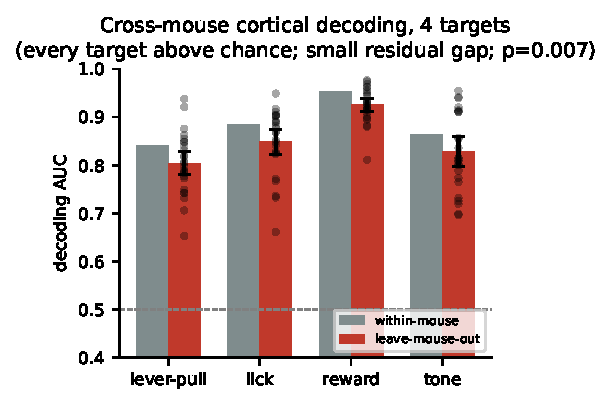
\includegraphics[width=0.7\linewidth]{figs/fig1_auc.pdf}
\caption{Within-mouse vs.\ leave-one-mouse-out $\auc$ for all four targets (bootstrap CI; dots =
held-out mice). Cross-animal decoding approaches the within-animal ceiling---a small residual gap.}
\label{fig:auc}\end{figure}

\subsection{Longitudinal stability of the cross-animal decoder}
\label{sec:drift}
Does the shared readout survive the passage of days? Using the four-regime design
(Table~\ref{tab:drift}, Fig.~\ref{fig:drift}), we find it does. First, there is no
\emph{within}-animal drift: training on days 1--5 and testing on days 11--15 of the same mouse
loses nothing (lever-pull WX $0.838$ vs.\ WS $0.826$; lick $0.865$ vs.\ $0.883$; CIs overlap).
Second, and centrally, the \emph{cross-animal} decoder is temporally stable: trained only on other
mice's first-week sessions and tested on a held-out mouse's \emph{last-week} sessions (LX), it
equals or exceeds the same-block cross-animal control (LS)---lever-pull $0.818$ vs.\ $0.792$
(paired $\Delta=+0.026$, sign-flip $p=0.008$, $n=25$) and lick $0.842$ vs.\ $0.832$ ($\Delta=+0.010$,
$p=0.45$). In no regime is the across-block decoder worse; the mildly positive direction is
consistent with late-week behavior being more practiced and thus slightly cleaner, not with
temporal degradation. Finally, a within-mouse train-day/test-day sweep ($>2300$ session pairs per
target) shows accuracy is flat in the day-gap: slopes are $-0.0004$ (lever-pull) and $-0.0022$
(lick) $\auc$/day, i.e.\ $<0.04$ $\auc$ lost across the entire two-week span
(Fig.~\ref{fig:drift}, right). The cross-animal behavioral code is thus stable along \emph{both} the
individual and the session axes.

\begin{table}[t]\centering
\caption{Longitudinal design: within/across-animal $\times$ same/across-block $\auc$. Training on
days 1--5 and testing on days 11--15---within a mouse or across mice---incurs no loss.}
\label{tab:drift}
\begin{tabular}{lcccc}
\toprule
 & \multicolumn{2}{c}{within-mouse} & \multicolumn{2}{c}{leave-one-mouse-out} \\
\cmidrule(lr){2-3}\cmidrule(lr){4-5}
Target & same (WS) & early$\to$late (WX) & same (LS) & early$\to$late (LX) \\
\midrule
Lever-pull & 0.826 & 0.838 & 0.792 & 0.818 \\
Lick       & 0.883 & 0.865 & 0.832 & 0.842 \\
\bottomrule
\end{tabular}
\end{table}

\begin{figure}[t]\centering
\begin{minipage}{0.56\linewidth}\centering
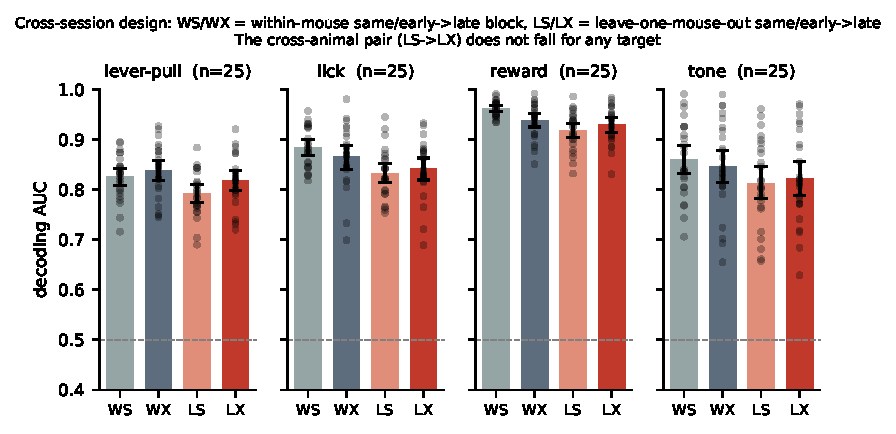
\includegraphics[width=\linewidth]{figs/fig4_drift_2x2.pdf}
\end{minipage}\hfill
\begin{minipage}{0.42\linewidth}\centering
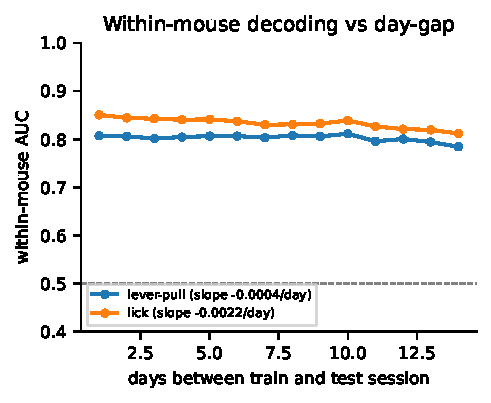
\includegraphics[width=\linewidth]{figs/fig5_daygap.pdf}
\end{minipage}
\caption{\textbf{Left:} within/across-animal $\times$ same/across-block decoding (bootstrap CI;
dots = mice); the conserved code is temporally stable. \textbf{Right:} within-mouse accuracy vs.\
train--test day-gap is flat (slopes $-0.0004$ and $-0.0022$ $\auc$/day).}
\label{fig:drift}\end{figure}

\subsection{Capacity-invariance: the gap does not grow with model capacity}
\label{sec:nl}
The linear baseline collapses each event to one evoked-difference vector, discarding temporal
dynamics. A higher-capacity model could exploit those dynamics---but it could also overfit
mouse-specific idiosyncrasies and \emph{open} a cross-animal gap. We test both by comparing the
linear model to a 1-D CNN and a GRU over the full window on identical events and splits
(Table~\ref{tab:nl}, Fig.~\ref{fig:nl}). Both temporal models raise absolute accuracy sharply:
cross-animal $\auc$ rises from $0.804$ to $0.895$/$0.909$ (CNN/GRU) for lever-pull and from
$0.850$ to $0.966$/$0.962$ for lick---a $+0.09$ to $+0.12$ gain, so the collapsed vector leaves
real signal in the dynamics unused. Crucially, the cross-subject gap does \emph{not} widen: LOMO
trails within-mouse by only $0.03$--$0.05$ $\auc$ for every model---no more for the high-capacity
temporal networks than for the linear one, and less for lick ($-0.013$ vs.\ $-0.036$). The shared
component of the code therefore includes the temporal response, not merely its mean; capacity buys
accuracy without costing transfer. (In this pooled-session regime a small gap is present even for
the linear model because within-mouse CV benefits from more per-mouse data than the single-session
analysis of Table~\ref{tab:main}; the point is that capacity does not enlarge it.)

\begin{table}[t]\centering
\caption{Linear vs.\ nonlinear temporal decoders. Temporal models are far more accurate, yet the
cross-subject gap (LOMO $-$ within) is no larger than the linear model's.}
\label{tab:nl}
\begin{tabular}{llccc}
\toprule
Target & Model & Within-mouse & LOMO & Gap \\
\midrule
\multirow{3}{*}{Lever-pull}
 & Linear (evoked)    & 0.842 & 0.804 & $-0.037$ \\
 & 1-D CNN (temporal) & 0.942 & 0.895 & $-0.047$ \\
 & GRU (temporal)     & 0.935 & 0.909 & $-0.026$ \\
\midrule
\multirow{3}{*}{Lick}
 & Linear (evoked)    & 0.886 & 0.850 & $-0.036$ \\
 & 1-D CNN (temporal) & 0.978 & 0.966 & $-0.013$ \\
 & GRU (temporal)     & 0.975 & 0.962 & $-0.013$ \\
\bottomrule
\end{tabular}
\end{table}

\begin{figure}[t]\centering
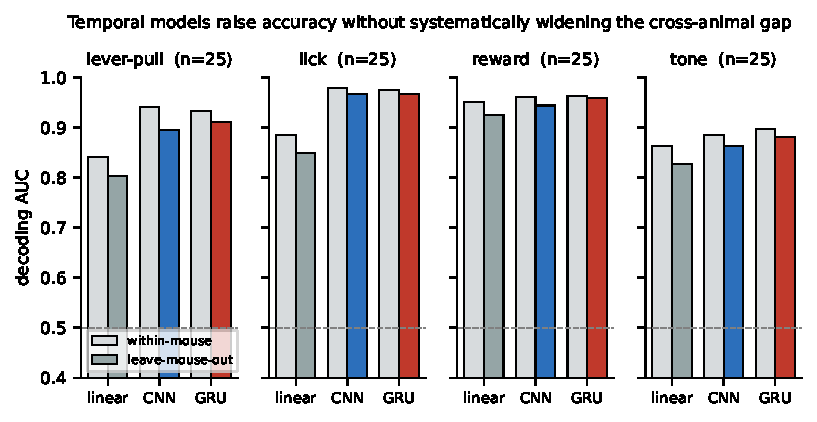
\includegraphics[width=0.9\linewidth]{figs/fig6_nonlinear.pdf}
\caption{Within-mouse vs.\ LOMO $\auc$ for the linear and two nonlinear temporal decoders.
Capacity raises accuracy markedly but does not open a cross-animal gap.}
\label{fig:nl}\end{figure}

\subsection{Cross-dataset replication and cortical localization}
\label{sec:repl}
\textbf{Replication.} To test dataset-specificity we repeat the analysis on an independent
widefield cohort from a different laboratory (Cardin--Higley; \citealp{benisty2024}; 6 mice, 23
CCFv3 parcels, \emph{spontaneous} behavior, different targets). Movement (locomotion) reaches LOMO
$\auc$ $0.731$ (within-mouse $0.744$) and arousal (pupil) $0.627$ (within $0.645$): the same
near-ceiling cross-animal readout (gap $0.01$--$0.02$) appears across a different lab, atlas, task,
and behavioral variable, indicating a general property of cortex rather than a cohort artifact.

\textbf{Localization.} Decoder weights (Fig.~\ref{fig:parcels}) are spatially structured and
dominated by high-amplitude midline cortex---retrosplenial (RSPagl, RSPd) and posterior
visual-association/parietal areas (VISam, VISa)---shared across all four targets, as expected when
a movement/arousal-related component pervades widefield activity \citep{musall2019}. Target
identity modulates the finer weighting: the tone (auditory-cue) and lick decoders additionally
recruit somatosensory (nose, upper-limb; SSp) and motor parcels that the reward decoder does not.
The codes thus carry target-specific structure over a shared backbone rather than being pure
generic arousal.

\begin{figure}[t]\centering

\includegraphics[width=0.92\linewidth]{figs/fig2_parcels.pdf}\\[4pt]
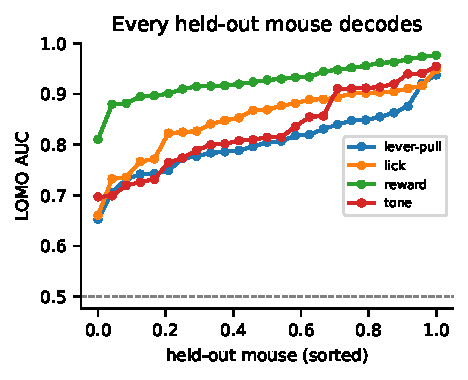
\includegraphics[width=0.6\linewidth]{figs/fig3_permouse.pdf}
\caption{\textbf{Top:} top Allen-atlas parcels by decoder weight---a shared midline
retrosplenial/visual-association backbone with target-specific somatosensory/motor modulation.
\textbf{Bottom:} per-held-out-mouse LOMO $\auc$ (sorted); every held-out mouse decodes above
chance.}
\label{fig:parcels}\end{figure}

\section{Discussion}
On BraiDyn-BC, cortex-wide representations of all four task events generalize to unseen individuals
within $0.03$--$0.04$ $\auc$ of within-animal decoding, and---our main contribution---that small
gap is \emph{stable across a 15-day protocol on both the within- and cross-animal axes} and
\emph{invariant to model capacity}. The shared component of the code is therefore invariant to
individual identity, to session, and to whether the decoder is a 44-parameter linear map or a
temporal network; and it includes the response dynamics, not only the collapsed evoked mean. That
cortex-wide dynamics are conserved across individuals is not itself new
\citep{macdowell2020,macdowell2024,musall2019}, and a concurrent foundation model performs
atlas-aligned cross-subject decoding on this cohort \citep{wicat2026}; our contribution is the
interpretable, near-ceiling, and longitudinally- and capacity-controlled characterization those
lines do not provide.

\textbf{Limitations.} We decode the four thresholdable task-event channels; continuous or graded
behavioral variables are a natural next target. Our conclusions rest on LOMO-vs-within and
across-vs-same-block \emph{comparisons} rather than absolute $\auc$, and they hold for both the
linear and the nonlinear decoders. The residual cross-animal gap is small but non-zero: we
characterize rather than eliminate it. The longitudinal-novelty framing is, to the best of our
literature search, unaddressed by prior work, but rests on absence of evidence; and the WiCAT
comparison is to a concurrent, non-archival preprint whose numbers may change.

\section{Conclusion}
A strict leave-one-mouse-out analysis in a shared 44-parcel atlas space shows that cortex-wide
widefield representations of four behavioral events are read out across unseen mice within
$0.03$--$0.04$ $\auc$ of the within-animal ceiling, and that this small cross-subject gap is
stable across a two-week protocol and invariant to decoder capacity, with an independent-cohort
replication. We release code and a streamed-feature pipeline that reproduces every number without
downloading raw imaging.

\subsubsection*{Reproducibility statement}
All data are open (BraiDyn-BC, DANDI:001425, CC-BY; Cardin--Higley, figshare 175317). We release
the full analysis code and a streaming feature pipeline that reproduces every table and figure
from the public parcellated traces without downloading raw widefield movies; all splits,
permutation seeds, and model hyperparameters are specified in Section 3 and the released code.

\bibliographystyle{plainnat}
\begin{thebibliography}{99}
\bibitem[Ajioka et al.(2024)]{ajioka2024} T.~Ajioka, N.~Nakai, O.~Yamashita, and T.~Takumi.
End-to-end deep learning approach to mouse behavior classification from cortex-wide calcium
imaging. \emph{PLOS Computational Biology}, 20(3):e1011074, 2024.
\bibitem[Benisty et al.(2024)]{benisty2024} H.~Benisty, A.~Lohani, D.~Barson, R.~C.~Cardin,
M.~J.~Higley, et al. Rapid fluctuations in functional connectivity of cortical networks encode
spontaneous behavior. \emph{Nature Neuroscience}, 27:148--158, 2024. Data: figshare project 175317.
\bibitem[Kondo et al.(2025)]{kondo2025} A.~Kondo et al. BraiDyn-BC: a cortex-wide widefield calcium
imaging dataset during a cued lever-pull operant task. \emph{Scientific Data}, 12, 2025.
DANDI:001425.
\bibitem[MacDowell \& Buschman(2020)]{macdowell2020} C.~J.~MacDowell and T.~J.~Buschman.
Low-dimensional spatiotemporal dynamics underlie cortex-wide neural activity. \emph{Current
Biology}, 30(14):2665--2680, 2020.
\bibitem[MacDowell et al.(2024)]{macdowell2024} C.~J.~MacDowell et al. Shared cortex-wide
spatiotemporal motifs govern activity across individuals and behavioral states. \emph{Current
Biology}, 34, 2024.
\bibitem[Melbaum et al.(2022)]{melbaum2022} S.~Melbaum et al. Conserved structures of neural
activity in sensorimotor cortex of freely moving rats enable cross-subject decoding. \emph{Nature
Communications}, 13:7902, 2022.
\bibitem[Musall et al.(2019)]{musall2019} S.~Musall, M.~T.~Kaufman, A.~L.~Juavinett, S.~Gluf, and
A.~K.~Churchland. Single-trial neural dynamics are dominated by richly varied movements.
\emph{Nature Neuroscience}, 22(10):1677--1686, 2019.
\bibitem[Rule et al.(2020)]{rule2020} M.~E.~Rule et al. Stable task information from an unstable
neural population. \emph{eLife}, 9:e51121, 2020.
\bibitem[Schneider et al.(2023)]{schneider2023} S.~Schneider, J.~H.~Lee, and M.~W.~Mathis.
Learnable latent embeddings for joint behavioural and neural analysis (CEBRA). \emph{Nature},
617:360--368, 2023.
\bibitem[Hosseini et al.(2026)]{wicat2026} S.~Hosseini et al. WiCAT: cross-subject modeling for
widefield calcium imaging via atlas-aligned spatiotemporal tokenization. \emph{arXiv preprint}
arXiv:2607.09754, 2026.
\end{thebibliography}

\end{document}
